\documentclass[a4paper,10pt]{article}

\usepackage{ucs}
\usepackage[utf8x]{inputenc}
\usepackage[english]{babel}
\usepackage{fontenc}
\usepackage{graphicx}
\usepackage[a4paper, top=2cm]{geometry}
\usepackage{amssymb}

\usepackage[dvips]{hyperref}
\title{String Algorithms 2013 - Assignment 3}
\author{Holger Schmeisky  201211113, Matus Tomlein 201210962}
\date{29.05.2013}

\begin{document}

\maketitle

\subsection*{State of the project}
Our algorithms work correctly and in the expected worst-case running time.

\subsection*{Insights}
\begin{itemize}
  \item we chose python because coding in it is less verbose than in java
  \item useful not to stick too close to pseudocode, think more about what needs to be done
\end{itemize}

\subsection*{Problems}
During the correctness evaluation we discovered another index error in the implementation. We accessed the shift-array one position too far back, because we did not align the indices properly.

\subsection*{Evaluation of correctness}

We created a script that evaluates the results of our KMP and BA algorithm
implementations and compares them against the results of a naive algorithm
that searches for a given pattern by comparing substrings at each index
in the given string.
We used a long DNA string as an input and generated random search patterns
based on the input string.

According to the evaluation, both our KMP and BA implementations worked
correctly.

\clearpage
\subsection*{Evaluation}

\subsection*{Comparison with suffix tree}

The question was:
\emph{How many times should you search for a pattern in the same text before it faster to use search from mandatory project 1 (based on constructing the suffix tree) rather than search-ba or search-kmp?}

As soon as searching for the pattern K times in BA and KMP takes longer
than constructing the suffix tree for the input, we can say that searching in
the suffix tree is more efficient.
If we store the suffix tree, we have to pay the cost of creating it only once,
afterwards searching for any pattern takes just $\mathcal{O}(M)$.
However, in KMP and BA it always takes $\mathcal{O}(M+N)$ to search for a pattern.


\subsection*{Evaluation}
We evaluated the worst-case running time of the algorithm by generating worst-case inputs and running them repeatedly to get a running time independent of invocation overhead and computer variance. We executed the experiment on one of our laptops.\\

A worst-case inputs for both algorithms is a text of all the same letters, for example "AAAAAAA" and a pattern of the same letters, but with a different one at the end, e.g. "AAB". For this input the algorithm actually has to scan all characters of the input text once, because it only mismatches on the last character of the pattern, and there the border is 0.
\begin{figure}
  \centering
  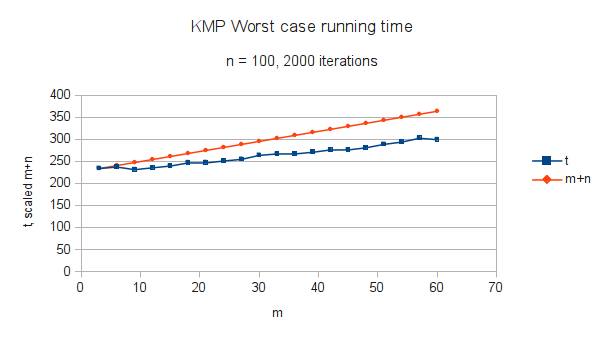
\includegraphics{./images/eval_kmp.png}
  % eval_kmp.pdf: 595x842 pixel, 72dpi, 20.99x29.70 cm, bb=0 0 595 842
  \label{fig:eval}
\end{figure}

\begin{figure}
  \centering
  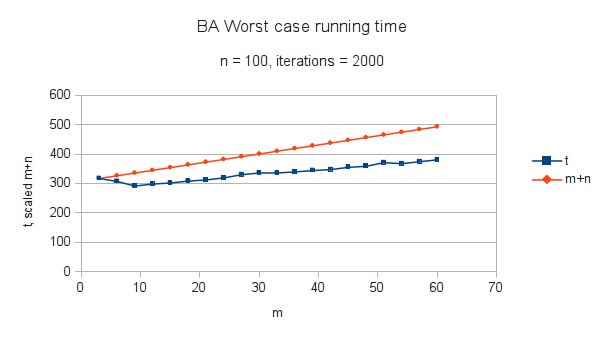
\includegraphics{./images/eval_ba - 1.png}
  % eval_kmp.pdf: 595x842 pixel, 72dpi, 20.99x29.70 cm, bb=0 0 595 842
  \label{fig:eval}
\end{figure}

\end{document}
